\documentclass[a4paper,12pt,oneside,pdflatex,final]{article}

% Core Packages
\usepackage[utf8]{inputenc}
\usepackage{siunitx}
\usepackage{booktabs}
\usepackage{fancyhdr}
\usepackage{graphicx}
\usepackage{float}
\usepackage{titlesec}
\usepackage{tabularx}
\usepackage{enumitem}
\usepackage{xcolor}
\usepackage[export]{adjustbox}
\usepackage[margin=0.7in]{geometry}

% Font settings
\usepackage{libertine}
\renewcommand*\familydefault{\sfdefault} 
\usepackage[T1]{fontenc}

% Brand Colors
\definecolor{brandblue}{HTML}{8594E8} 
% Custom section formatting
\titleformat{\section}
  {\color{brandblue}\normalfont\Large\bfseries}{\thesection}{1em}{}[{\titlerule[0.8pt]}]

% Header/Footer setup
\pagestyle{fancy}
\fancyhf{}
\lhead{\textbf{RPi CM5 Interface Board}}
\chead{Datasheet v1.1.0}
\rhead{\today}
\rfoot{Page \thepage}

\begin{document}

% --- TITLE HEADER ---
\begin{figure}[h!]
    \begin{minipage}[c]{0.55\textwidth}
        \raggedright
        {\color{brandblue}\Huge \textbf{RPi CM5 Interface Board}} \\[0.2cm]
        {\Large Breakout board for the Raspberry Pi Compute Module 5} \\[0.15cm]
        {\large \textcolor{brandblue}{\textbf{Board Version 1.1.0}}} \\[0.4cm]
        
        \textbf{\large Features}
        \begin{itemize}[leftmargin=*, nosep]
            \item Safe RPi Shutdown
            \item Status LEDs
            \item Programmable RGB LED
            \item IMU (Bosch BHI260AP)
            \item SD Card Slot
            \item Real-Time Clock
            \item Test Points
        \end{itemize}
    \end{minipage}
    \hfill
    \begin{minipage}[c]{0.4\textwidth}
        \raggedleft
        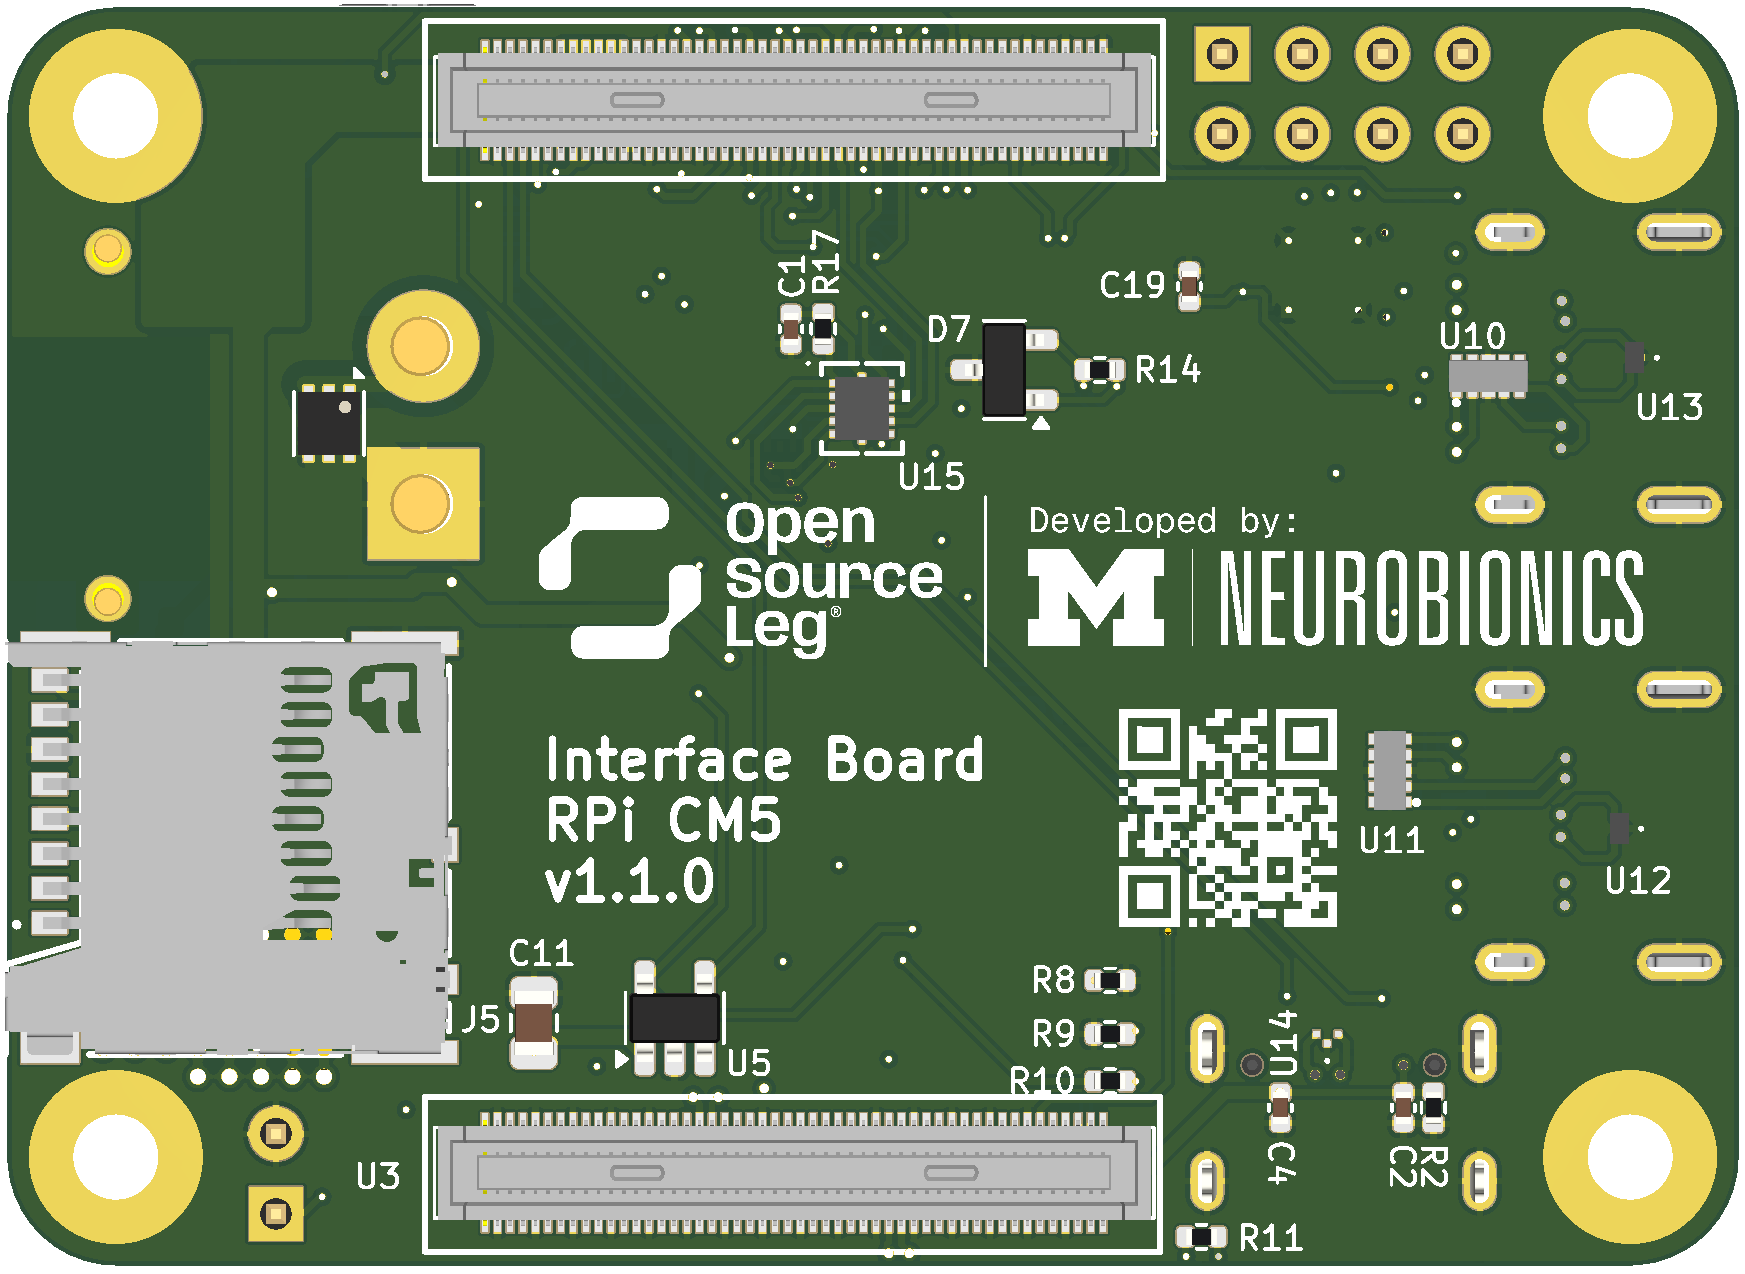
\includegraphics[width=0.95\textwidth]{pcb-front.png}
    \end{minipage}
\end{figure}


% --- OVERVIEW ---
\section{Overview}
The \textbf{RPi CM5 Interface Board} is an add-on module for the Raspberry Pi Compute Module 5 (RPi CM5) that is designed to provide plug and play functionality for sensors and actuators across a wide variety of robotics applications. It is built and tested by researchers at the University of Michigan's Neurobionics Lab.

% --- TECHNICAL SPECS ---
\section{Technical Specifications}
\begin{table}[h!]
    \centering
    \renewcommand{\arraystretch}{1.3}
    \begin{tabularx}{\textwidth}{l X}
    \toprule
    \textbf{Category} & \textbf{Specification} \\
    \midrule
    \textbf{Module Support} & Raspberry Pi Compute Module 5 (CM5) / CM5 Lite \\
    \textbf{Input Voltage} & 15V -- 53V (XT-30 Connector) | 5V (USB-C)\\
    \textbf{Power Output} & 5V @ 5A (SMPS) | 3.3V @ 1A (LDO) \\
    \textbf{USB Interface} & 2x USB-C 3.0 (High-Speed Communication) \\
    \textbf{CAN Bus} & 2x CAN Bus (MCP2515 Controller + MCP2562 Transceiver) \\
    \textbf{Sensors} & Bosch BHI260AP (6-Axis IMU) on SPI0 chip select 1 \\
    \textbf{Storage} & MicroSD Card Slot (for CM5 Lite boot/storage) \\
    \textbf{Cooling} & 4-Pin Fan Connector (PWM Control + Tachometer) \\
    \textbf{Dimensions} & $55.00\,\si{mm} \times 40.00\,\si{mm} \times 14.09\,\si{mm}$ \\
    \bottomrule
    \end{tabularx}
\end{table}
% --- PINOUTS ---
\section{Pinout \& Interfaces}

\begin{minipage}[t]{0.48\textwidth}

    % =======================
    % UART-1
    % =======================
    \subsection*{UART-1 (Molex PicoClasp, 4-Pin)}
    \begin{minipage}[t]{0.60\textwidth}
        \begin{tabularx}{\textwidth}{c X}
        \toprule
        \textbf{Pin} & \textbf{Function} \\
        \midrule
        1 & +3.3V \\
        2 & UART1\_TX \\
        3 & UART1\_RX \\
        4 & GND \\
        \bottomrule
        \end{tabularx}
    \end{minipage}%
    \hfill
    \begin{minipage}[t]{0.35\textwidth}
        \centering
        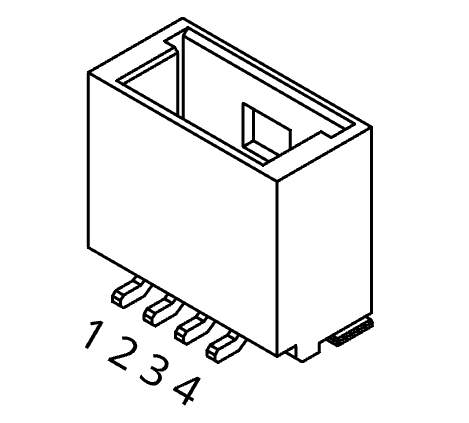
\includegraphics[width=\linewidth]{4pin_pico.png}
    \end{minipage}

    \vspace{0.6cm}

    % =======================
    % UART-2
    % =======================
    \subsection*{UART-2 (Molex PicoClasp, 4-Pin)}
    \begin{minipage}[t]{0.60\textwidth}
        \begin{tabularx}{\textwidth}{c X}
        \toprule
        \textbf{Pin} & \textbf{Function} \\
        \midrule
        1 & +3.3V \\
        2 & UART2\_TX \\
        3 & UART2\_RX \\
        4 & GND \\
        \bottomrule
        \end{tabularx}
    \end{minipage}%
    \hfill
    \begin{minipage}[t]{0.35\textwidth}
        \centering
        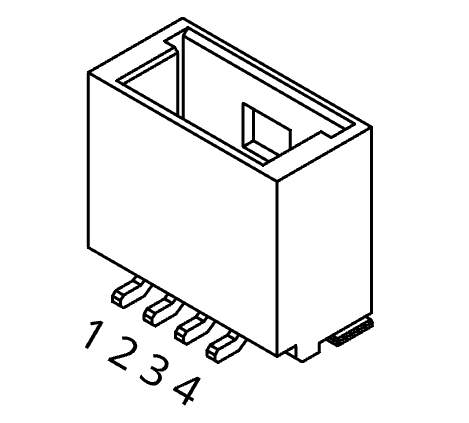
\includegraphics[width=\linewidth]{4pin_pico.png}
    \end{minipage}

    \vspace{0.6cm}

    % =======================
    % I2C-2
    % =======================
    \subsection*{I2C-2 (Molex PicoClasp, 4-Pin)}
    \begin{minipage}[t]{0.60\textwidth}
        \begin{tabularx}{\textwidth}{c X}
        \toprule
        \textbf{Pin} & \textbf{Function} \\
        \midrule
        1 & +3.3V \\
        2 & I2C2\_SDA \\
        3 & I2C2\_SCL \\
        4 & GND \\
        \bottomrule
        \end{tabularx}
    \end{minipage}%
    \hfill
    \begin{minipage}[t]{0.35\textwidth}
        \centering
        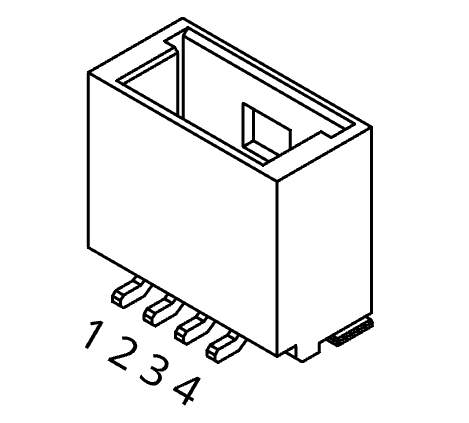
\includegraphics[width=\linewidth]{4pin_pico.png}
    \end{minipage}

    % =======================
    % I2C-3
    % =======================
    \subsection*{I2C-3 (Molex PicoClasp, 4-Pin)}
    \begin{minipage}[t]{0.60\textwidth}
        \begin{tabularx}{\textwidth}{c X}
        \toprule
        \textbf{Pin} & \textbf{Function} \\
        \midrule
        1 & +3.3V \\
        2 & I2C3\_SDA \\
        3 & I2C3\_SCL \\
        4 & GND \\
        \bottomrule
        \end{tabularx}
    \end{minipage}%
    \hfill
    \begin{minipage}[t]{0.35\textwidth}
        \centering
        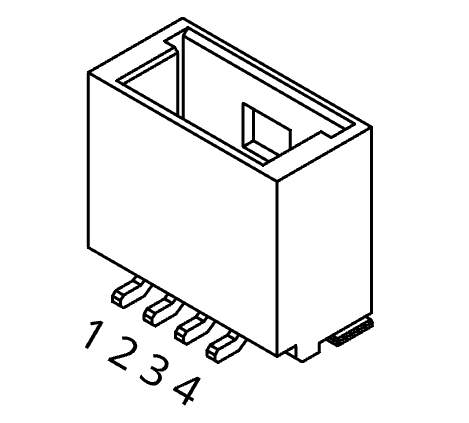
\includegraphics[width=\linewidth]{4pin_pico.png}
    \end{minipage}

    \vspace{0.6cm}
\end{minipage}
\hfill
\begin{minipage}[t]{0.48\textwidth}
    % =======================
    % SPI-1
    % =======================
    \subsection*{SPI-1 (Molex PicoClasp, 8-Pin)}
    \begin{minipage}[t]{0.60\textwidth}
        \begin{tabularx}{\textwidth}{c X}
        \toprule
        \textbf{Pin} & \textbf{Function} \\
        \midrule
        1 & +3.3V \\
        2 & SPI1\_CSn2 \\
        3 & SPI1\_CSn1 \\
        4 & SPI1\_CSn0 \\
        5 & SPI1\_SCLK \\
        6 & SPI1\_MISO \\
        7 & SPI1\_MOSI \\
        8 & GND \\
        \bottomrule
        \end{tabularx}
    \end{minipage}%
    \hfill
    \begin{minipage}[t]{0.35\textwidth}
        \centering
        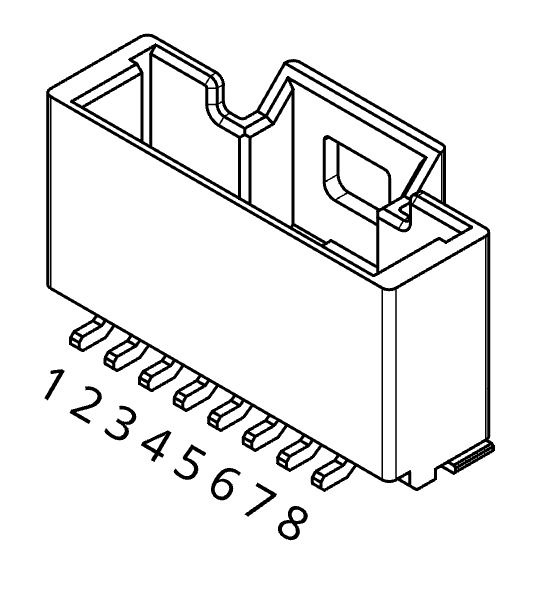
\includegraphics[width=\linewidth]{8pin_pico.png}
    \end{minipage}

    \vspace{0.6cm}

    % =======================
    % CAN
    % =======================
    \subsection*{CAN-0/1 (Molex PicoClasp), 3-Pin)}
    \begin{minipage}[t]{0.60\textwidth}
        \begin{tabularx}{\textwidth}{c X}
        \toprule
        \textbf{Pin} & \textbf{Function} \\
        \midrule
        1 & GND \\
        2 & CAN\_P \\
        3 & CAN\_N \\
        \bottomrule
        \end{tabularx}
    \end{minipage}%
    \hfill
    \begin{minipage}[t]{0.35\textwidth}
        \centering
        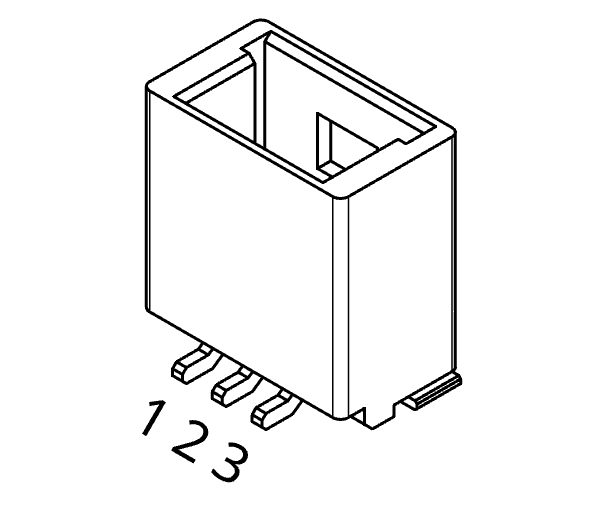
\includegraphics[width=\linewidth]{3pin_pico.png}
    \end{minipage}

    % =======================
    % GPIO Headers
    % =======================
    \subsection*{GPIO HEADERS}
    \begin{minipage}[t]{0.60\textwidth}
        \begin{tabularx}{\textwidth}{c X}
        \toprule
        \textbf{Pin} & \textbf{Function} \\
        \midrule
        1 & GPIO\_25\\
        2 & GPIO\_23\\
        3 & GPIO\_7\\
        4 & +3.3V\\
        5 & GPIO\_27\\
        6 & GPIO\_24\\
        7 & GPIO\_22\\
        8 & GND\\
        \bottomrule
        \end{tabularx}
    \end{minipage}%
    \hfill
    \begin{minipage}[t]{0.35\textwidth}
        \centering
        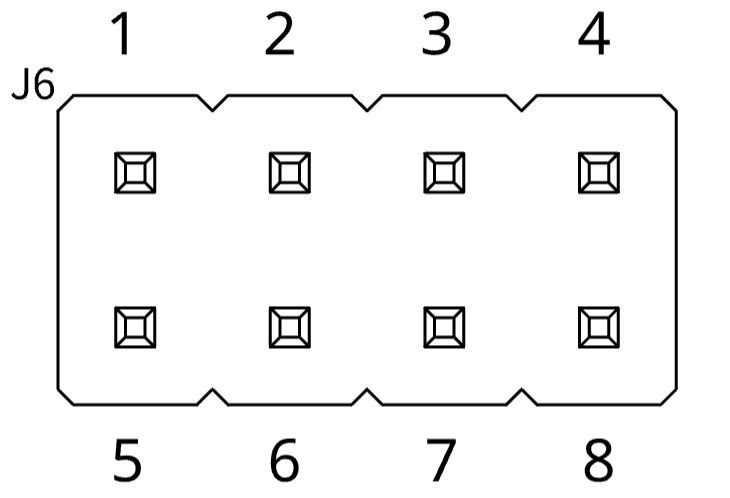
\includegraphics[width=\linewidth]{pinheader_number.png}
    \end{minipage}

    % =======================
    % Fan Port
    % =======================
    \subsection*{Fan Port, JST 4-Pin Connector}
    \begin{minipage}[t]{0.60\textwidth}
        \begin{tabularx}{\textwidth}{c X}
        \toprule
        \textbf{Pin} & \textbf{Function} \\
        \midrule
        1 & Tachometer\\
        2 & GND\\
        3 & PWM\\
        4 & +5V\\
        \bottomrule
        \end{tabularx}
    \end{minipage}%
    \hfill
    \begin{minipage}[t]{0.35\textwidth}
        \centering
        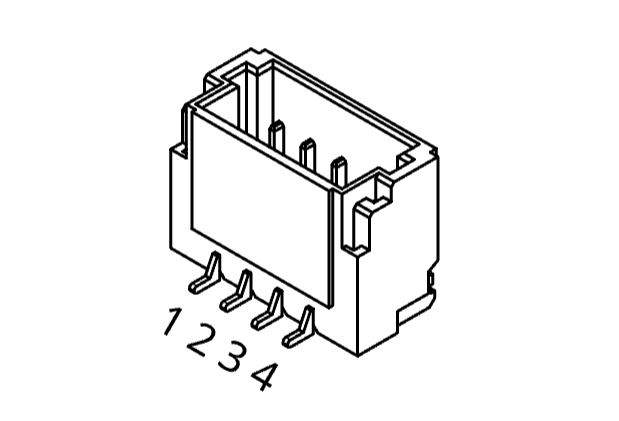
\includegraphics[width=\linewidth]{fanport_numbering.png}
    \end{minipage}

\end{minipage}

\hfill

\clearpage
% --- MECHANICAL ---
\section{Mechanical Details}
\begin{itemize}
    \item \textbf{PCB Dimensions:} $55\,\si{mm} \times 40\,\si{mm}$
    \item \textbf{Mounting Holes:} $4\times 2.7\,\si{mm}$ (Standard M2.5)
    \item \textbf{Max Height:} $14.09\,\si{mm}$ (Top of USB-C connector to bottom pins)
\end{itemize}

\begin{figure}[h!]
    \centering
    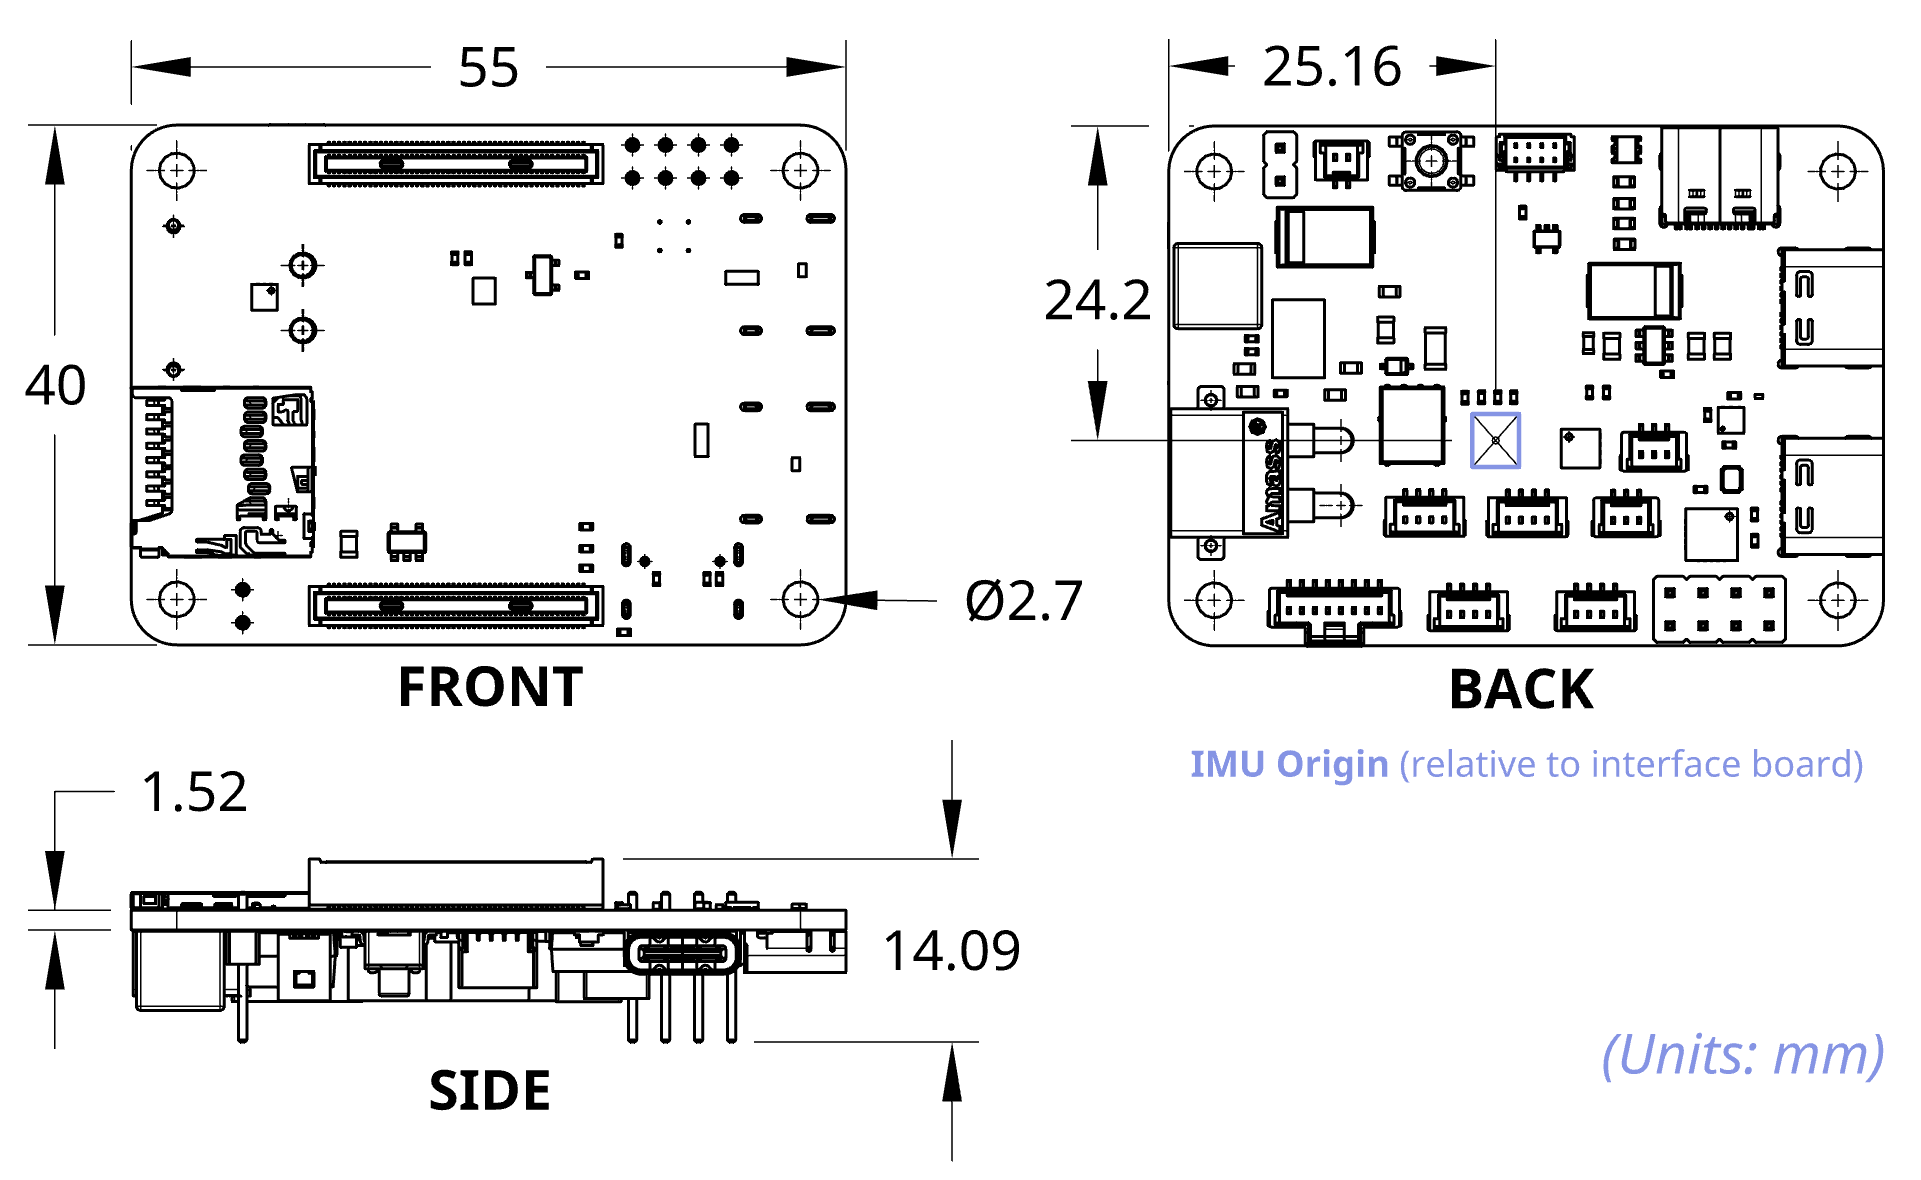
\includegraphics[width=0.9\textwidth]{mechanical_specs.png}
    \caption{Mechanical Drawing \& Sensor Origin}
\end{figure}

% Other components
\section{Other Components}

\begin{itemize}[leftmargin=*]
    \item \textbf{Signal LEDs:} 5V, 3.3V, Power, and Activity
    \item \textbf{Programmable RGB LED:} Addressable RGB LED for user feedback and debugging

    \item \textbf{J4 External Switch:} Can be used for safe RPi shutdown with an external switch using a Molex PicoClasp 2-pin connector
    \item \textbf{Safe Shutdown Circuit:} Allows clean shutdown of the Raspberry Pi without power corruption

    \item \textbf{Real-Time Clock (RTC):} Maintains system time when RPi is off (only interface board is powered).

    \item \textbf{Test Points:} Labeled test points for power rails and key signals to assist debugging
    \item \textbf{Boot Configuration Access:} Hardware support for CM5 boot and bring-up workflows
\end{itemize}


\end{document}